%------------------------------------------------
\section{Заключение}
%------------------------------------------------
\begin{frame}
	\frametitle{Благодарность}
	\begin{center}
		Спасибо за внимание!
	\end{center}
	
\end{frame}
%------------------------------------------------
\begin{frame}
	\begin{center}
		Back up
	\end{center}
\end{frame}
%------------------------------------------------
\begin{frame}
	\frametitle{Подавление дисперсии}
	\begin{figure}
		\centering
		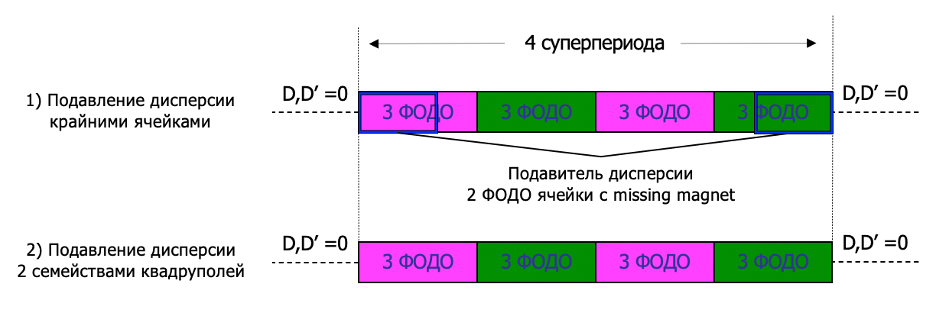
\includegraphics[width=0.8\linewidth]{images/2_disp_supp_shemes}
	\end{figure}
\end{frame}
%------------------------------------------------
\begin{frame}
	\frametitle{Критическая энергия}
	Уравнения продольного движения:
	\begin{equation}
		\begin{cases}
			\begin{aligned}
				& \dv{\tau}{t}=\eta(\delta) \cdot \frac{h \cdot \Delta E}{\beta^2 \cdot E_0} \\
				& \dv{(\Delta E)}{t}=\frac{V(\tau)}{T_0}
			\end{aligned}
		\end{cases}
		\label{eq:long_motion_eq_t}
	\end{equation}	
	Коэффициент уплотнения орбиты (momentum compaction factor):
	\begin{equation}
		\alpha_c=\frac{1}{C_0} \dv{C}{\delta}=\alpha_0+2 \alpha_1 \delta+3 \alpha_2 \delta^2+\cdots \equiv \frac{1}{\gamma_{\textrm{tr}}^2} = \frac{1}{C} \int_0^{\mathrm{C}} \frac{D(s)}{\rho(s)} d s,
		\label{eq:alpha}
	\end{equation}
	Коэффициент проскальзывания (slip-factor):
	\begin{equation}
		\eta = \eta_{0} = \alpha_{0} - \frac{1}{\gamma_{0}^2}.
		\label{eq:slip-factor_0}
	\end{equation}
\end{frame}
%------------------------------------------------
\begin{frame}
	\frametitle{Суперпериодическая модуляция}
	Уравнение для дисперсионной функции с бипериодической переменной фокусировкой
	\begin{equation}
		\dv[2]{D}{s}+\left[K(s)+\varepsilon k(s)\right]D=\frac{1}{\rho(s)} ,
		\label{eq:disp_eq}
	\end{equation}
	MCF для одного суперпериода в первом приближении
	\begin{equation}
		\begin{aligned}
			\alpha_s= & \frac{1}{\nu^2}\left\{1+\frac{1}{4(1-k S / \nu)}\left(\frac{\bar{R}}{\nu}\right)^4 \frac{g_k^2}{\left[1-(1-k S / \nu)^2\right]^2}\right\}.
		\end{aligned}
		\label{eq:alpha_gradient}
	\end{equation}
	\begin{figure}
		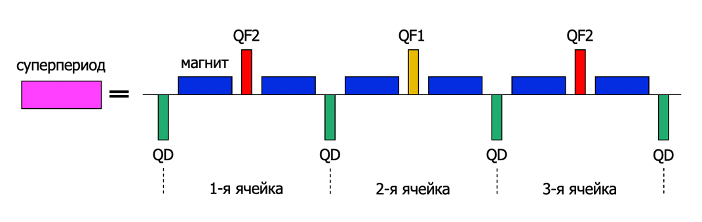
\includegraphics[width=0.6\linewidth]{images/2_superperiod}
	\end{figure}
\end{frame}
%------------------------------------------------
\begin{frame}
	\frametitle{Оптимальное время жизни пучка}
	Временная эволюция эмиттанса и разброса импульса в присутствии процессов охлаждения
	\begin{equation}
		\dv{\varepsilon}{t} =\underbrace{-\frac{1}{\tau_{\text{tr}}} \cdot \varepsilon}_{\text{cooling}}+\underbrace{\left(\dv{\varepsilon}{t}\right)_{\text{IBS}}}_{\text{heating}}, \quad
		\dv{\delta^2}{t} =\underbrace{-\frac{1}{\tau_{\text{long}}} \cdot \delta^2}_{\text{cooling}}+\underbrace{\left(\dv{\delta^2}{t}\right)_{\text{IBS}}}_{\text{heating}}.
	\end{equation}
	Для независимых от времени, стационарных значений, производные по времени становятся равными нулю
	\begin{equation}
		\varepsilon_{\textrm{st}}=\left.\tau_{\text{tr}} \cdot\left(\dv{\varepsilon}{t}\right)_{\text{IBS}}\right|_{\varepsilon=\varepsilon_{\text{st}}}, \quad
		\delta_{st}^2=\left.\tau_{\text{long}} \cdot\left(\dv{\delta^2}{t}\right)_{\text{IBS}}\right|_{\delta^2=\delta_{\text{st}}^2}.
	\end{equation}
\end{frame}
%------------------------------------------------
\begin{frame}
	\frametitle{Прохождение критической энергии}
	Характерное время \textit{адиабатичности} и \textit{нелинейность} продольного движения
	\begin{equation}
		\tau_{\textrm{ad}}=\left(\frac{\pi\beta^2mc^2\gamma_{\textrm{tr}}^4}{\dot{\gamma}\omega_0^2heV\left|\cos{\phi_{\textrm{s}}}\right|}\right)^{1/3}; \quad\quad
		\tau_{\textrm{nl}}=\frac{\eta_1\hat{\delta}}{\frac{2\dot{\gamma}}{{\gamma_{\textrm{tr}}}^3}}=\gamma_{\textrm{tr}}\frac{\frac{3}{2}\beta^2+\gamma_{\textrm{tr}}^2\alpha_1}{2\dot{\gamma}}\
	\end{equation}
	
	\begin{figure}
		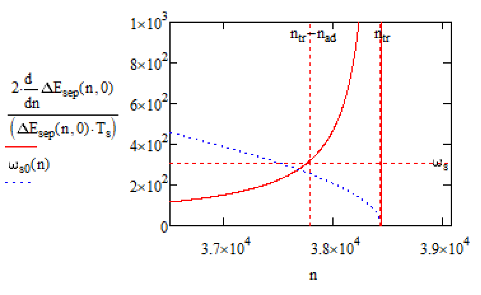
\includegraphics[width=0.4\columnwidth]{3_adiabatic_time.png}
		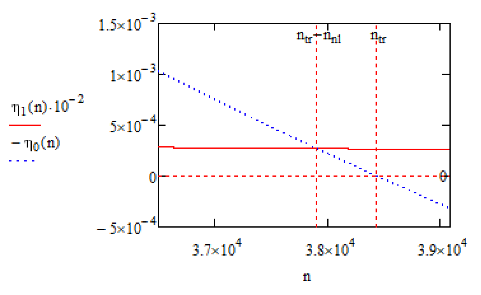
\includegraphics[width=0.4\columnwidth]{3_nonlin_time.png}
	\end{figure}
\end{frame}
%------------------------------------------------
\begin{frame}
	\frametitle{Моделирование динамики}
	\centering
	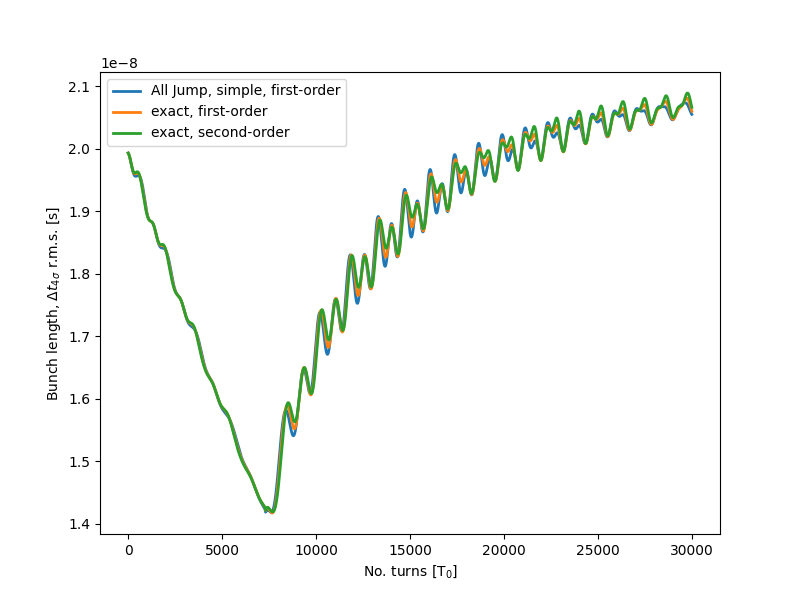
\includegraphics[width=0.275\columnwidth]{3_jump_beam_lenght.png}
	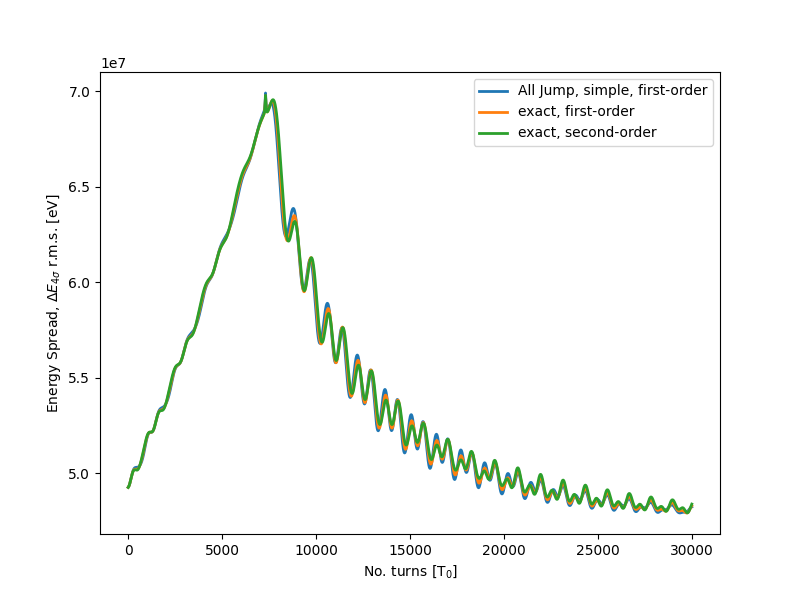
\includegraphics[width=0.275\columnwidth]{3_jump_energy_spread.png}
	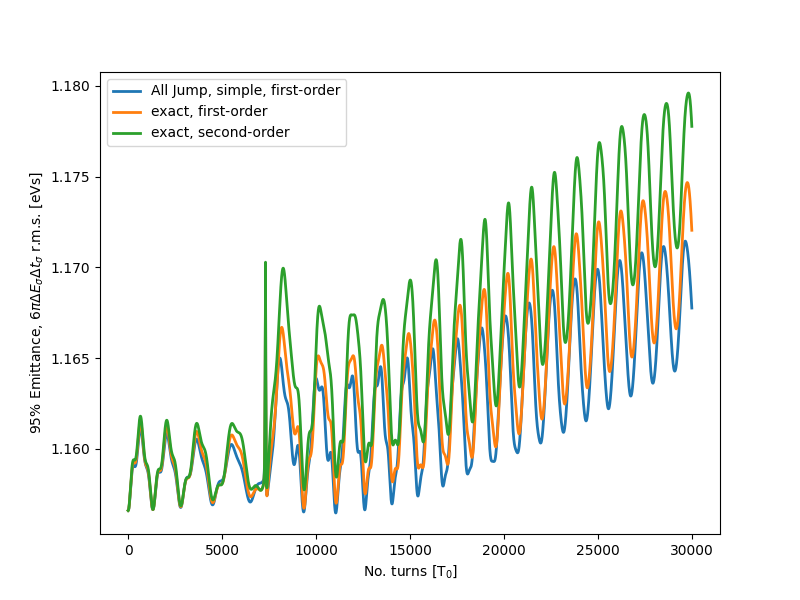
\includegraphics[width=0.275\columnwidth]{3_jump_emit.png}
	
	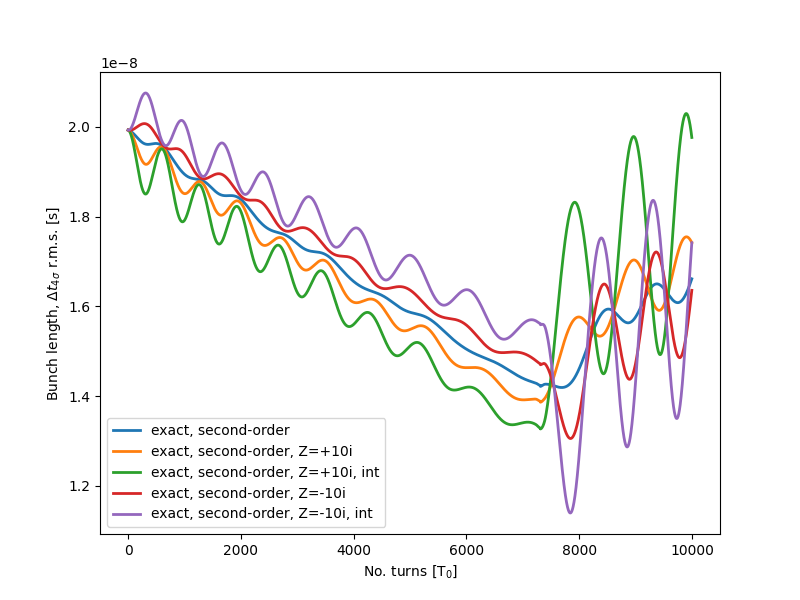
\includegraphics[width=0.275\columnwidth]{3_jump_imp_beam_lenght.png}
	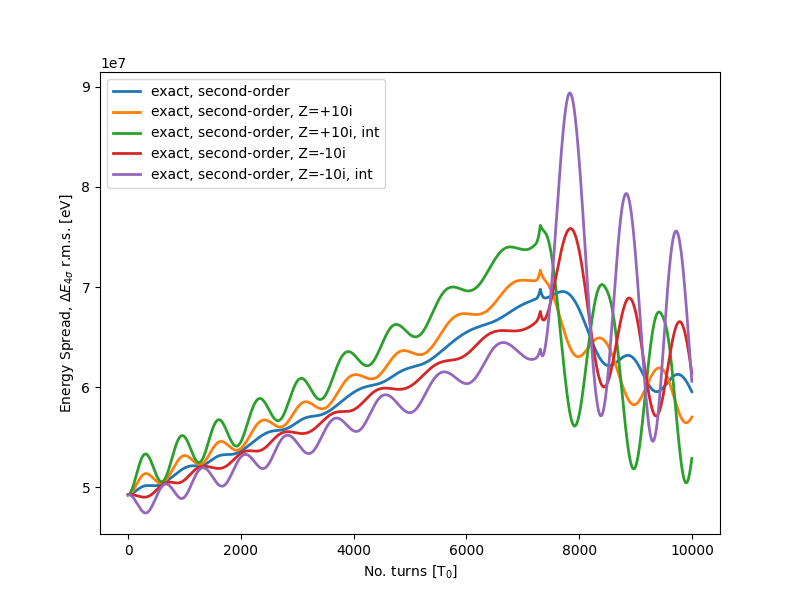
\includegraphics[width=0.275\columnwidth]{3_jump_imp_energy_spread.png}
	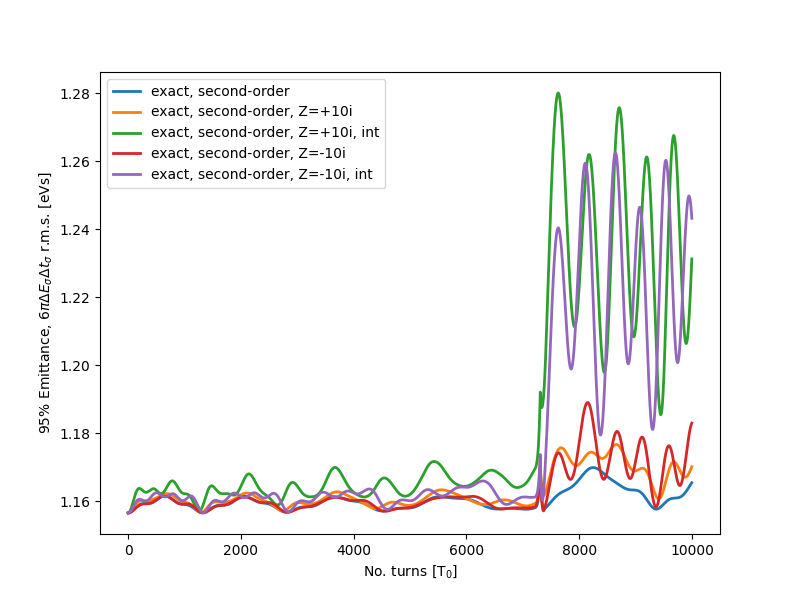
\includegraphics[width=0.275\columnwidth]{3_jump_imp_emit.png}
\end{frame}
%------------------------------------------------
\begin{frame}
	\frametitle{Скачок критической энергии в гармоническом ВЧ}
	\centering
	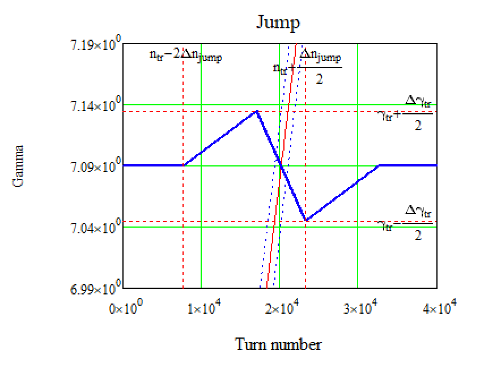
\includegraphics[width=0.4\columnwidth]{3_g_tr_harmonic.png}
	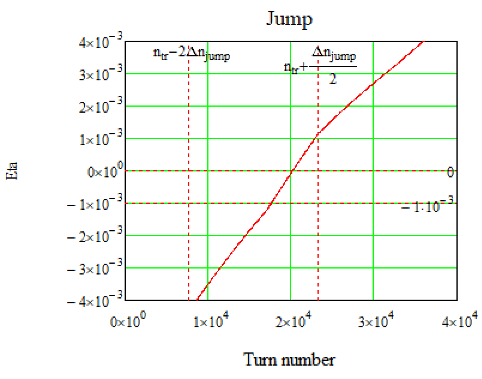
\includegraphics[width=0.4\columnwidth]{3_eta_tr_harmonic.png}
\end{frame}
%------------------------------------------------
\begin{frame}
	\frametitle{Скачок критической энергии в барьерном ВЧ I}
	\centering
	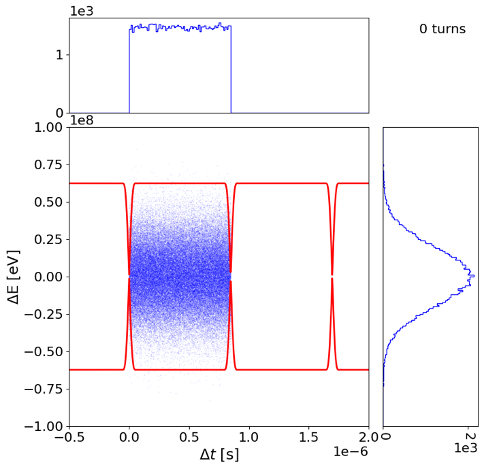
\includegraphics[width=.4\columnwidth]{3_BB_PS_near_tr}
	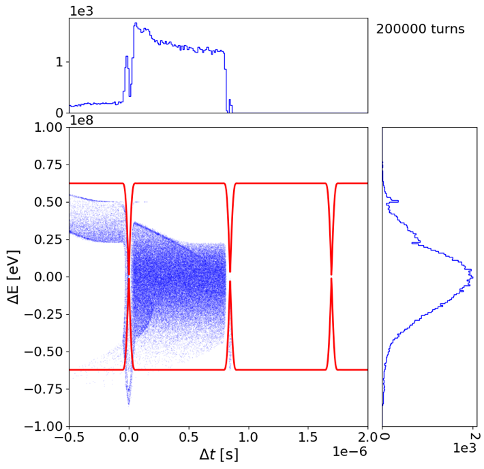
\includegraphics[width=.4\columnwidth]{3_BB_PS_near_tr_2}
\end{frame}
%------------------------------------------------
\begin{frame}
	\frametitle{Скачок критической энергии в барьерном ВЧ II}
	\centering
	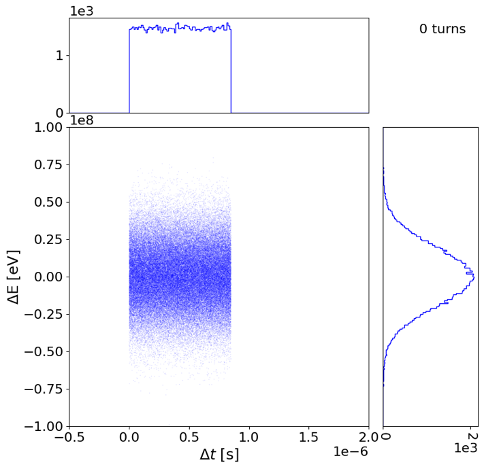
\includegraphics[width=.4\columnwidth]{3_BB_PS_jump}
	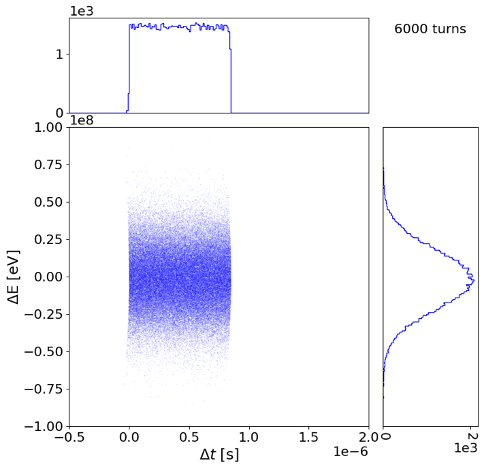
\includegraphics[width=.4\columnwidth]{3_BB_PS_jump_2}
\end{frame}
%------------------------------------------------
\begin{frame}
	\frametitle{Влияние импеданса}
	\centering
	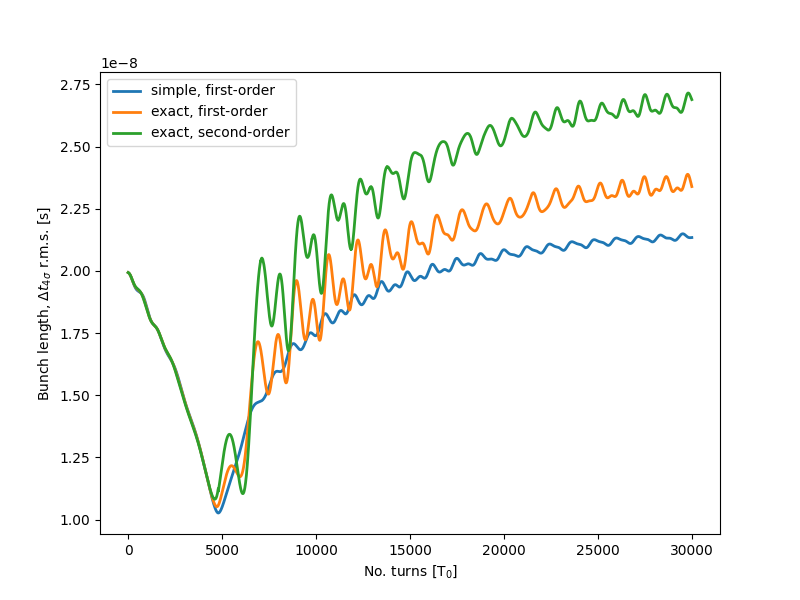
\includegraphics[width=0.275\columnwidth]{3_eta_beam_lenght.png}
	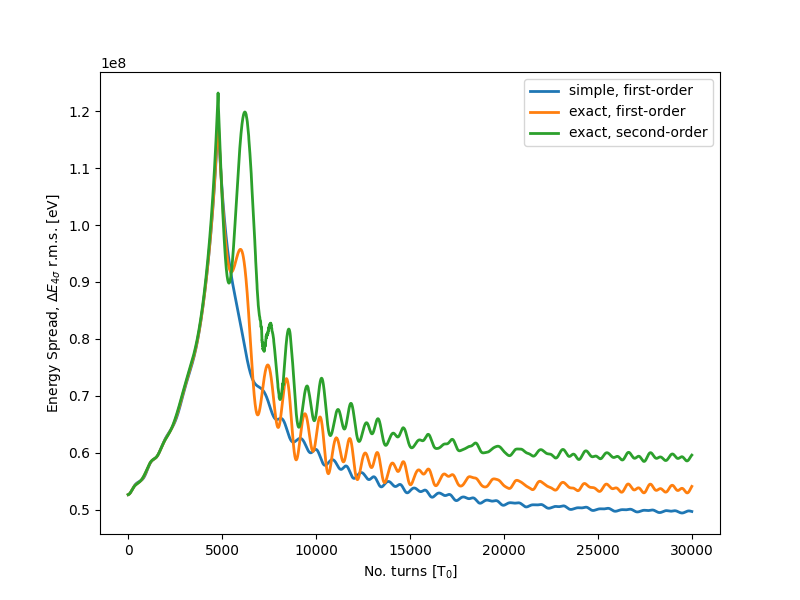
\includegraphics[width=0.275\columnwidth]{3_eta_energy_spread.png}
	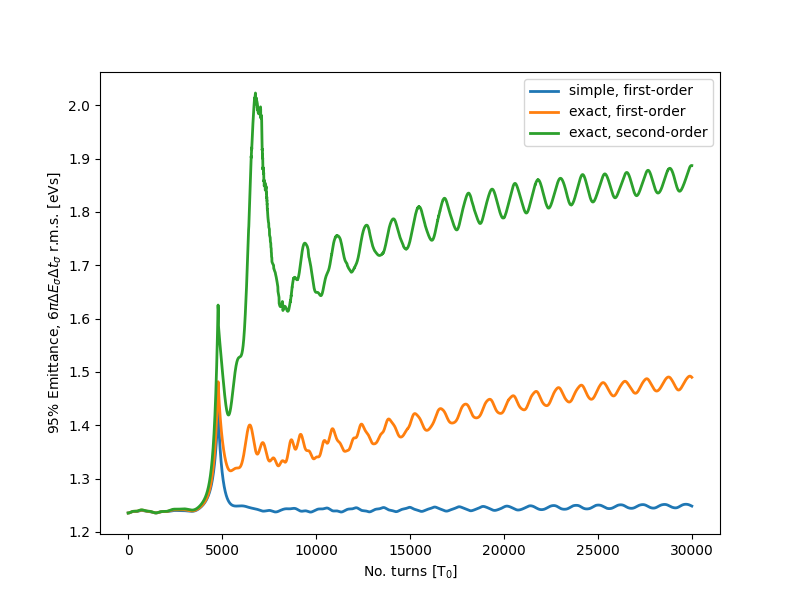
\includegraphics[width=0.275\columnwidth]{3_eta_emit.png}
	
	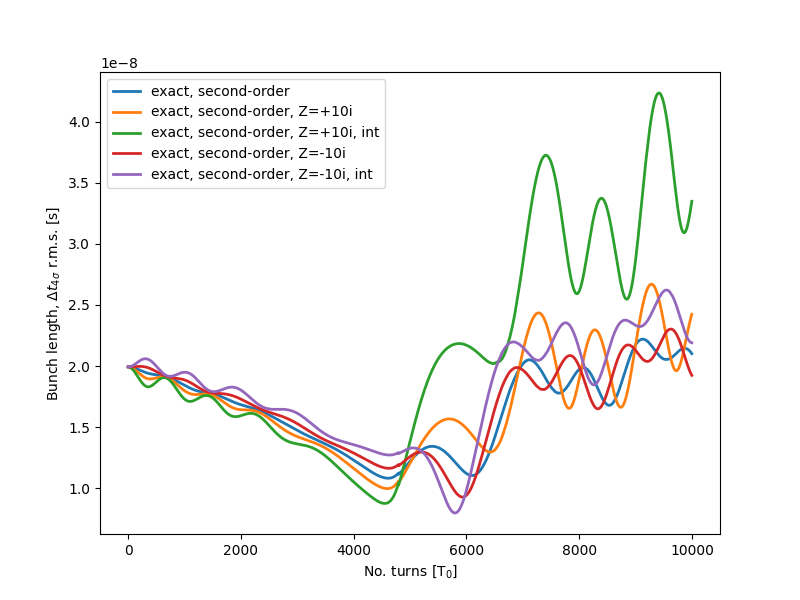
\includegraphics[width=0.275\columnwidth]{3_wo_jump_beam_lenght.png}
	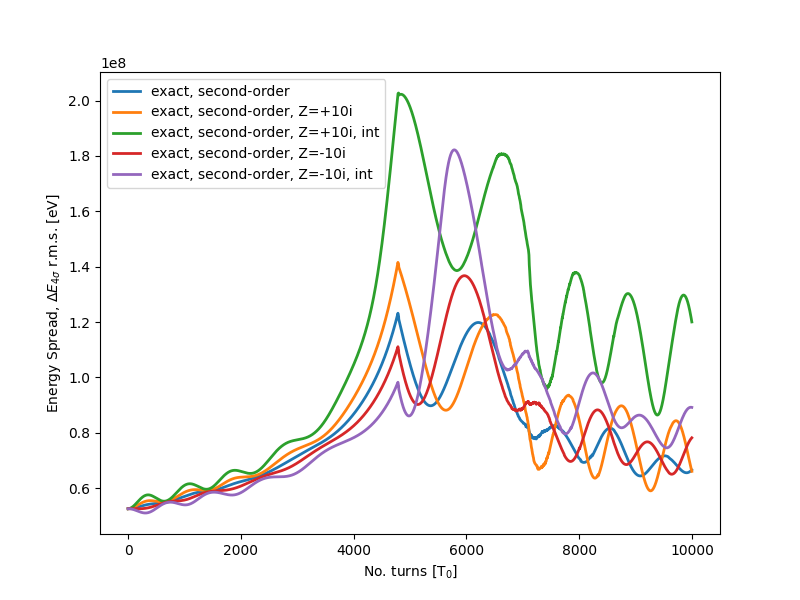
\includegraphics[width=0.275\columnwidth]{3_wo_jump_energy_spread.png}
	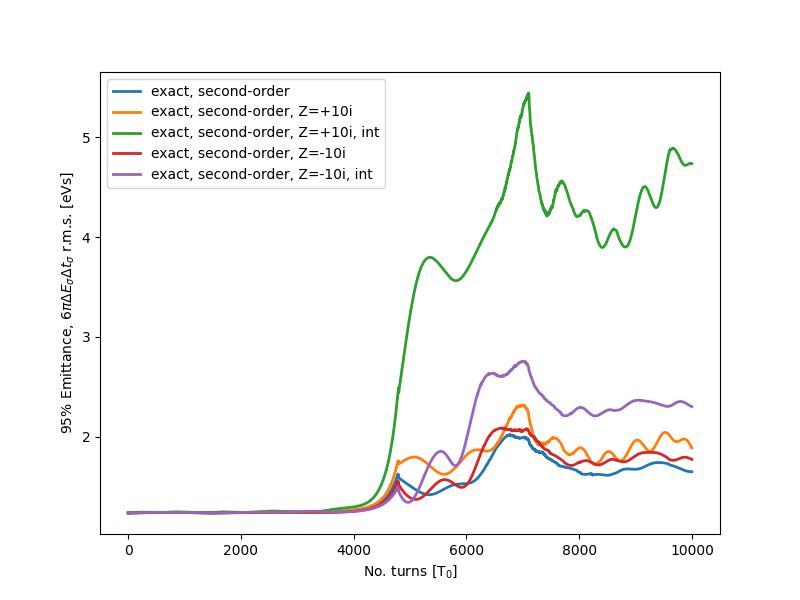
\includegraphics[width=0.275\columnwidth]{3_wo_jump_emit.png}
\end{frame}
%------------------------------------------------
\begin{frame}
	\frametitle{Модернизация Nuclotron 8-ми периодическая структура}
	\centering
	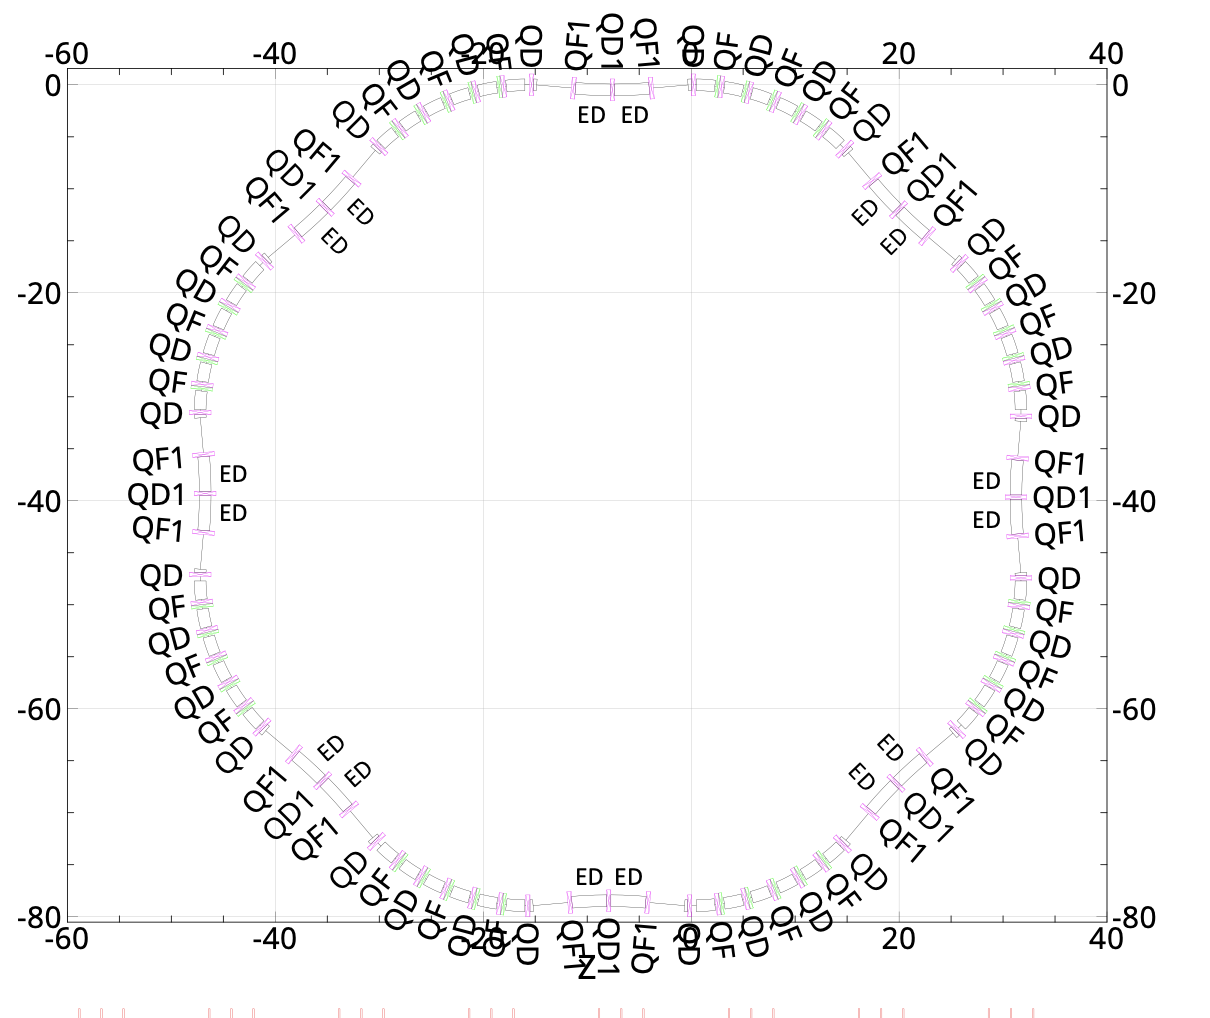
\includegraphics[width=0.45\columnwidth]{4_Nuclotron_8_def1.png}
	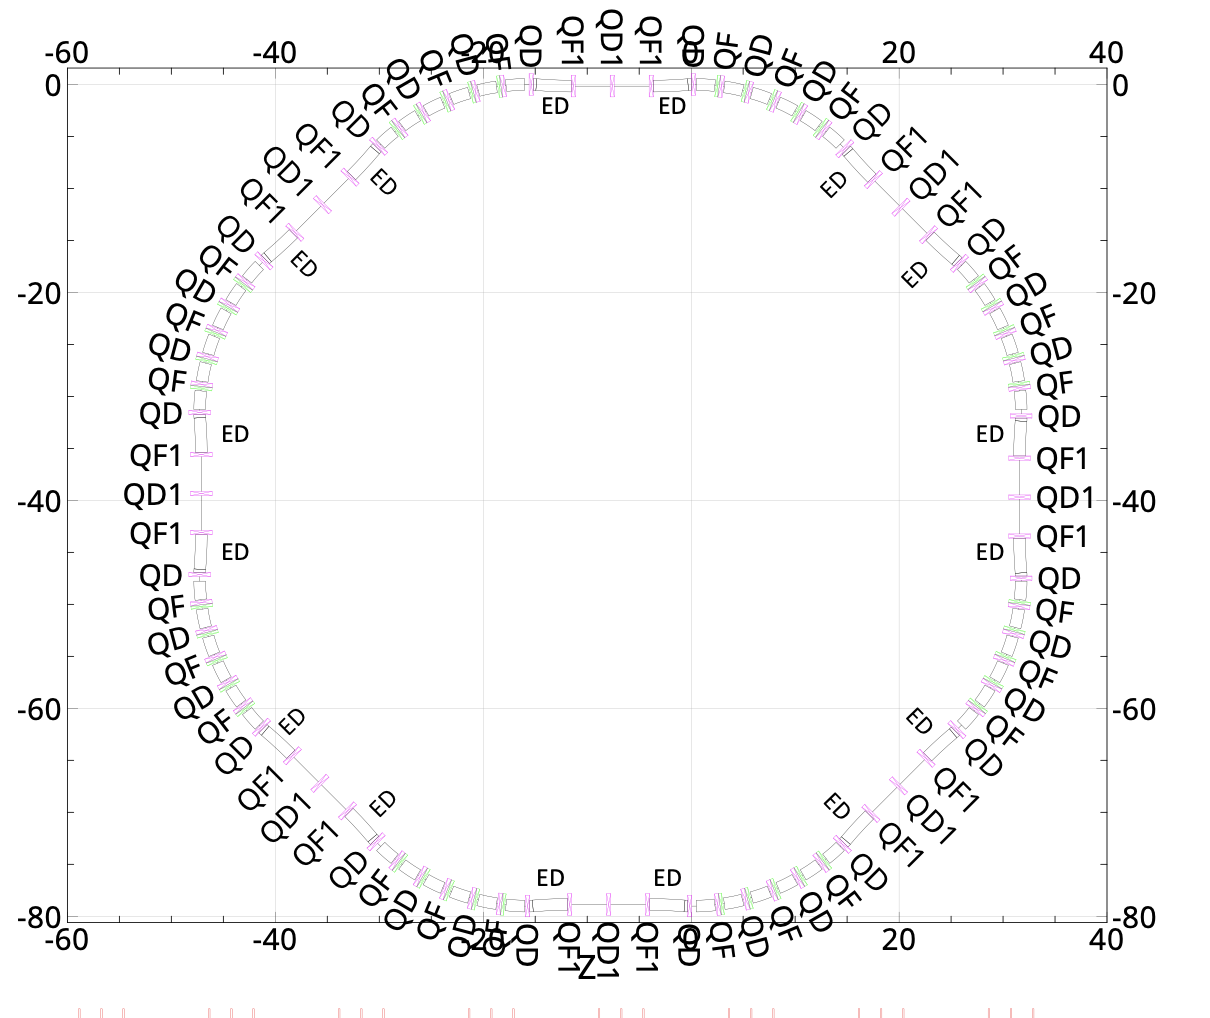
\includegraphics[width=0.45\columnwidth]{4_Nuclotron_8_def2.png}
\end{frame}
%------------------------------------------------